\chapter{Programmazione Lineare Mista}

\section{Enunciazione}

\begin{align*}
    opt \;\; f(x) = c^Tx \\
    X = \begin{Bmatrix} x : g_i(x) \begin{Bmatrix} \geq \\ = \\ \leq \end{Bmatrix} 0, i = 1,...,m \end{Bmatrix} &\land g_i(x) = a_i^T - b_i \\
    a \in \R^n, b \in \R^n, c \in \R^n, opt = \begin{Bmatrix} min \\ max \end{Bmatrix}
\end{align*}

\begin{itemize}
    \item Se $x \in \Z^n$ allora abbiamo un problema di \textbf{Programmazione Lineare Intera} (PLI)
    \item Se $x \in \{0,1\}^n$ allora abbiamo un problema di \textbf{Programmazione Lineare Binaria} (PB)
    \item Se $x \in \R^p \times \Z^q$ allora abbiamo un problema di \textbf{Programmazione Lineare Mista} (PLM o MIP)
\end{itemize}

\section{Variabili Binarie}

Risolvono problemi nella modellazione del problema:
\begin{itemize}
    \item Un problema decisionale del tipo Si'/No, es: Devo costruire o no una fabbrica a Gragnano Trebbiense?
    \item Un problema di selezione di siti o beni, es: Quale percorso o bene devo scegliere per un servizio?
    \item Un problema di tempistiche, es: Quando devo cominciare una certa attivita'? \\
\end{itemize}

Ma servono anche per includere particolari condizioni. \\

\paragraph{Vincoli di tipo Either-Or}

Ho due vincoli $f(x) \leq F$, $g(x) \leq G$ e sono uno dei due vincoli deve essere soddisfatto.
Creo una variabile binaria $y \in \{0,1\}$, considero poi una variabile $M = +\infty$ e formulo il problema cosi:

\[
    \begin{cases}
        f(x) \leq F + My \\
        g(x) \leq G + M(1-y)
    \end{cases}
\]

In questo modo se y = 1, allora f(x) sara' sempre soddisfatta e rimarra' selezionata g(x) e vice versa.

\paragraph{K Vincoli su N}

Dati N vincoli solo K devono essere veri.
La modellazione simile alla precedente.

\[
    \begin{cases}
        f_1(x) \leq F_1 + My_1 \\
        f_2(x) \leq F_2 + My_2 \\
        f_3(x) \leq F_3 + My_3 \\
         ... \\
        f_n(x) \leq F_n + My_n \\
        \Sigma^N_{i=1} y_i = N - K \\
    \end{cases}
\]

\paragraph{N possibili valori}

Nel caso in cui un vincolo abbia una risorsa con piu' di un valore possibile.
Creo N variabili binarie $y_i$, corrispondente alle N risorse $d_i$.

\[
    \begin{cases}
        f(x) = \Sigma^N_{i=1} d_i y_i
        \Sigma^N_{i=1} y_i = 1
    \end{cases}
\]

\paragraph{Costo fisso}

Se avessi una funzione di costo di una attivita' j formulata cosi':

\[
    f(x) = 
    \begin{cases}
        k + cx & x > 0\\
        0 & x = 0
    \end{cases}
\]

La minimizzazione di questa funzione sarebbe la seguente:

\[
    min \; z = (ky + cx)
    \begin{cases}
        x - My \leq 0 \\
        y \in \{0,1\} \land x >= 0
    \end{cases}
\]

\paragraph{Rappresentazione binaria di variabili intere}

Voglio rappresentare x, che so essere nel range [0,u], chiamo N quell'intero tale che $2^N \leq u \leq 2^{N+1}$.
Quindi scrivo x = $\Sigma ^N _{i=0} 2^i y_i$.

\section{Risoluzione}

I problemi di Programmazione Lineare Intera e Binaria non possono essere risolti in modo piu' semplice rispetto alla Programmazione Lineare con Simplesso, anzi sono piu' complessi.

\paragraph{Rilassamento Lineare}

I problemi richiedono di subire un Rilassamento Lineare, una trasformazione che li "approssima" a problemi di Programmazione Lineare. \\

Una variabile $x \in \Z$ viene trasformata in:
\[
    \begin{cases}
    x \geq 0
    \end{cases}
\]

Una variabile $x \in \{0,1\}$ viene trasformata in:
\[
    \begin{cases}
        x \leq 1 \\
        x \geq 0
    \end{cases}
\]

\paragraph{Simplesso}

Quindi si calcola il simplesso del problema rilassato, e si controlla se la soluzione ottimale e' intera. Se non lo e' non e' possibile approssimare con efficacia questa soluzione in intera.

\section{Matrice Totalmente Unimodulare}

Una matrice si dice Totalmente Unimodulare (TUM) se $det(Q) \in \{1,0,-1\}$ per ogni sua sottomatrice quadrata, di qualunque ordine.

\paragraph{Caso particolare}

Sia A una matrice tale che $\forall i,j \in A \mid a_{ij} \in \{1,0,-1\}$ e tale che ogni colonna ha al più due elementi diversi da zero discordi.
Questa e' una condizione sufficiente ma non necessaria per asserire che e' una matrice TUM.

esempio preso da slide di A. Gobbi:

\begin{center}
    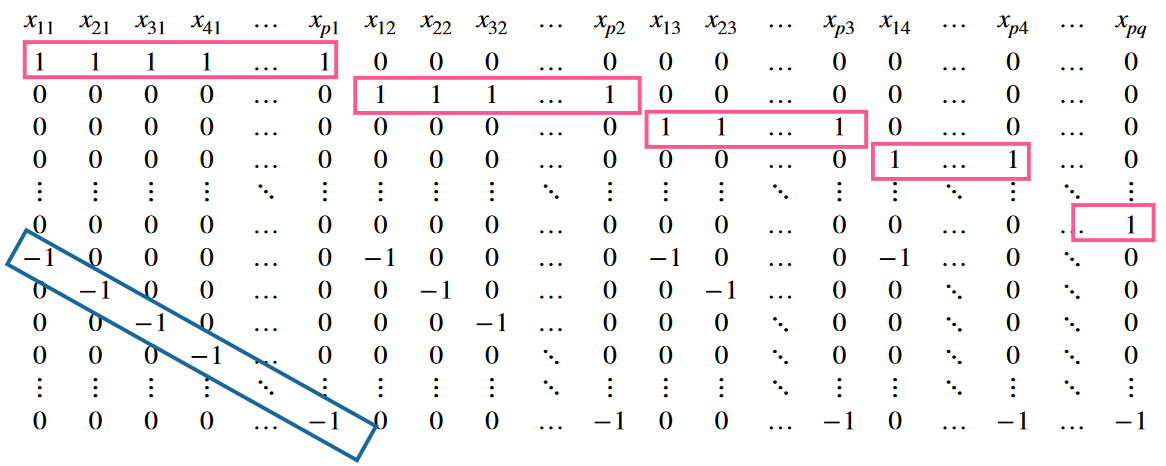
\includegraphics[width=12cm]{images/teoria/programmazione-lineare-mista/TUM.png}
\end{center}

\section{TUM Interezza}

Sia $A$ una matrice TUM e $b$ un intero. Il Poliedro $Ax \geq b \cap x \geq 0$ ha solo vertici interi.
Quindi ogni sua soluzione ottimale e' automaticamente intera!

\section{TUM Binarieta'}

Il rilassamento lineare di una variabile binaria porta ai seguenti vincoli
\[
    \begin{cases}
        x \leq 1 \\
        x \geq 0
    \end{cases}
\]

Quindi $1 \geq x \geq 0$. Se vale la TUM Interezza allora $x \in \Z$. \\
Questo assicura che x sia binaria, infatti $1 \geq x \geq 0 \land x \in \Z \Leftrightarrow x \in \{0,1\}$
